% Options for packages loaded elsewhere
\PassOptionsToPackage{unicode}{hyperref}
\PassOptionsToPackage{hyphens}{url}
%
\documentclass[
  man,floatsintext]{apa7}
\usepackage{amsmath,amssymb}
\usepackage{lmodern}
\usepackage{iftex}
\ifPDFTeX
  \usepackage[T1]{fontenc}
  \usepackage[utf8]{inputenc}
  \usepackage{textcomp} % provide euro and other symbols
\else % if luatex or xetex
  \usepackage{unicode-math}
  \defaultfontfeatures{Scale=MatchLowercase}
  \defaultfontfeatures[\rmfamily]{Ligatures=TeX,Scale=1}
\fi
% Use upquote if available, for straight quotes in verbatim environments
\IfFileExists{upquote.sty}{\usepackage{upquote}}{}
\IfFileExists{microtype.sty}{% use microtype if available
  \usepackage[]{microtype}
  \UseMicrotypeSet[protrusion]{basicmath} % disable protrusion for tt fonts
}{}
\makeatletter
\@ifundefined{KOMAClassName}{% if non-KOMA class
  \IfFileExists{parskip.sty}{%
    \usepackage{parskip}
  }{% else
    \setlength{\parindent}{0pt}
    \setlength{\parskip}{6pt plus 2pt minus 1pt}}
}{% if KOMA class
  \KOMAoptions{parskip=half}}
\makeatother
\usepackage{xcolor}
\usepackage{graphicx}
\makeatletter
\def\maxwidth{\ifdim\Gin@nat@width>\linewidth\linewidth\else\Gin@nat@width\fi}
\def\maxheight{\ifdim\Gin@nat@height>\textheight\textheight\else\Gin@nat@height\fi}
\makeatother
% Scale images if necessary, so that they will not overflow the page
% margins by default, and it is still possible to overwrite the defaults
% using explicit options in \includegraphics[width, height, ...]{}
\setkeys{Gin}{width=\maxwidth,height=\maxheight,keepaspectratio}
% Set default figure placement to htbp
\makeatletter
\def\fps@figure{htbp}
\makeatother
\setlength{\emergencystretch}{3em} % prevent overfull lines
\providecommand{\tightlist}{%
  \setlength{\itemsep}{0pt}\setlength{\parskip}{0pt}}
\setcounter{secnumdepth}{-\maxdimen} % remove section numbering
% Make \paragraph and \subparagraph free-standing
\ifx\paragraph\undefined\else
  \let\oldparagraph\paragraph
  \renewcommand{\paragraph}[1]{\oldparagraph{#1}\mbox{}}
\fi
\ifx\subparagraph\undefined\else
  \let\oldsubparagraph\subparagraph
  \renewcommand{\subparagraph}[1]{\oldsubparagraph{#1}\mbox{}}
\fi
\newlength{\cslhangindent}
\setlength{\cslhangindent}{1.5em}
\newlength{\csllabelwidth}
\setlength{\csllabelwidth}{3em}
\newlength{\cslentryspacingunit} % times entry-spacing
\setlength{\cslentryspacingunit}{\parskip}
\newenvironment{CSLReferences}[2] % #1 hanging-ident, #2 entry spacing
 {% don't indent paragraphs
  \setlength{\parindent}{0pt}
  % turn on hanging indent if param 1 is 1
  \ifodd #1
  \let\oldpar\par
  \def\par{\hangindent=\cslhangindent\oldpar}
  \fi
  % set entry spacing
  \setlength{\parskip}{#2\cslentryspacingunit}
 }%
 {}
\usepackage{calc}
\newcommand{\CSLBlock}[1]{#1\hfill\break}
\newcommand{\CSLLeftMargin}[1]{\parbox[t]{\csllabelwidth}{#1}}
\newcommand{\CSLRightInline}[1]{\parbox[t]{\linewidth - \csllabelwidth}{#1}\break}
\newcommand{\CSLIndent}[1]{\hspace{\cslhangindent}#1}
\ifLuaTeX
\usepackage[bidi=basic]{babel}
\else
\usepackage[bidi=default]{babel}
\fi
\babelprovide[main,import]{english}
% get rid of language-specific shorthands (see #6817):
\let\LanguageShortHands\languageshorthands
\def\languageshorthands#1{}
\usepackage{tabu}
\usepackage{amsmath}
\usepackage{setspace}
\AtBeginEnvironment{tabular}{\singlespacing}
\AtBeginEnvironment{lltable}{\singlespacing}
\AtBeginEnvironment{tablenotes}{\singlespacing}
\captionsetup[table]{font={stretch=1.5}}
\captionsetup[figure]{font={stretch=1.5}}
\usepackage{float} 
\floatplacement{figure}{H} 
\usepackage[font=sf]{caption}
\usepackage[fontsize=11.5pt]{fontsize} 
\newenvironment{fignote}{\begin{quote}\footnotesize}{\end{quote}}
\setlength{\textfloatsep}{10pt plus 3pt minus 5pt}
\usepackage{ragged2e}
\usepackage{parskip}
\parindent=0.5in
\setlength{\headsep}{0pt}
\setlength{\parskip}{0em}

\usepackage{blindtext}

\renewcommand*{\thepage}{\footnotesize\arabic{page}}
% Manuscript styling
\usepackage{upgreek}
\captionsetup{font=singlespacing,justification=justified}

% Table formatting
\usepackage{longtable}
\usepackage{lscape}
% \usepackage[counterclockwise]{rotating}   % Landscape page setup for large tables
\usepackage{multirow}		% Table styling
\usepackage{tabularx}		% Control Column width
\usepackage[flushleft]{threeparttable}	% Allows for three part tables with a specified notes section
\usepackage{threeparttablex}            % Lets threeparttable work with longtable

% Create new environments so endfloat can handle them
% \newenvironment{ltable}
%   {\begin{landscape}\centering\begin{threeparttable}}
%   {\end{threeparttable}\end{landscape}}
\newenvironment{lltable}{\begin{landscape}\centering\begin{ThreePartTable}}{\end{ThreePartTable}\end{landscape}}

% Enables adjusting longtable caption width to table width
% Solution found at http://golatex.de/longtable-mit-caption-so-breit-wie-die-tabelle-t15767.html
\makeatletter
\newcommand\LastLTentrywidth{1em}
\newlength\longtablewidth
\setlength{\longtablewidth}{1in}
\newcommand{\getlongtablewidth}{\begingroup \ifcsname LT@\roman{LT@tables}\endcsname \global\longtablewidth=0pt \renewcommand{\LT@entry}[2]{\global\advance\longtablewidth by ##2\relax\gdef\LastLTentrywidth{##2}}\@nameuse{LT@\roman{LT@tables}} \fi \endgroup}

% \setlength{\parindent}{0.5in}
% \setlength{\parskip}{0pt plus 0pt minus 0pt}

% Overwrite redefinition of paragraph and subparagraph by the default LaTeX template
% See https://github.com/crsh/papaja/issues/292
\makeatletter
\renewcommand{\paragraph}{\@startsection{paragraph}{4}{\parindent}%
  {0\baselineskip \@plus 0.2ex \@minus 0.2ex}%
  {-1em}%
  {\normalfont\normalsize\bfseries\itshape\typesectitle}}

\renewcommand{\subparagraph}[1]{\@startsection{subparagraph}{5}{1em}%
  {0\baselineskip \@plus 0.2ex \@minus 0.2ex}%
  {-\z@\relax}%
  {\normalfont\normalsize\itshape\hspace{\parindent}{#1}\textit{\addperi}}{\relax}}
\makeatother

% \usepackage{etoolbox}
\makeatletter
\patchcmd{\HyOrg@maketitle}
  {\section{\normalfont\normalsize\abstractname}}
  {\section*{\normalfont\normalsize\abstractname}}
  {}{\typeout{Failed to patch abstract.}}
\patchcmd{\HyOrg@maketitle}
  {\section{\protect\normalfont{\@title}}}
  {\section*{\protect\normalfont{\@title}}}
  {}{\typeout{Failed to patch title.}}
\makeatother

\usepackage{xpatch}
\makeatletter
\xapptocmd\appendix
  {\xapptocmd\section
    {\addcontentsline{toc}{section}{\appendixname\ifoneappendix\else~\theappendix\fi\\: #1}}
    {}{\InnerPatchFailed}%
  }
{}{\PatchFailed}
\usepackage{csquotes}
\ifLuaTeX
  \usepackage{selnolig}  % disable illegal ligatures
\fi
\IfFileExists{bookmark.sty}{\usepackage{bookmark}}{\usepackage{hyperref}}
\IfFileExists{xurl.sty}{\usepackage{xurl}}{} % add URL line breaks if available
\urlstyle{same} % disable monospaced font for URLs
\hypersetup{
  pdftitle={Examining contextual cueing using real-world scenes},
  pdfauthor={PsyBSc14 Grundlagen der Psychologie Vertiefung: Allgemeine Psycholgie I Jan Luca Schnatz Goethe University: Institut of Psychology Supervisor: M.Sc. Aylin Kallmayer Contact: s2787063@stud.uni-frankfurt.de November 2nd 2022},
  pdflang={en-EN},
  hidelinks,
  pdfcreator={LaTeX via pandoc}}

\title{Examining contextual cueing using real-world scenes}
\author{PsyBSc14 Grundlagen der Psychologie Vertiefung: Allgemeine Psycholgie I \break Jan Luca Schnatz \break Goethe University: Institut of Psychology \break Supervisor: M.Sc. Aylin Kallmayer \break Contact: \href{mailto:s2787063@stud.uni-frankfurt.de}{\nolinkurl{s2787063@stud.uni-frankfurt.de}} \break November 2nd 2022\textsuperscript{}}
\date{}


\shorttitle{\phantom{test}}

\affiliation{\phantom{0}}

\begin{document}
\maketitle

\newpage

\hypertarget{introduction}{%
\section{Introduction}\label{introduction}}

Humans are constantly exposed to an overloading flood of visual information competing for our attention, yet we are able to direct our attention precisely and quickly to targets that are relevant to goal-oriented behavior. This is rooted to a significant extent in the ability to harness the oftentimes stable and structured context of a scene by perceiving the invariant spatial arrangement between different objects in the environment and a target of interest. For example, if you search for your favorite psychology textbook in your tidy bookshelf, the book is located in a fixed location relative to the familiar environment (i.e.~the other books). The use of this contextual information in an invariant structure of the visual environment increases the predictability of the target location. To put it another way, the spatial configuration of a scene cues the location of the target, thus facilitating visual search (Chun, 2000).

These properties of the attentional system have been coined as \emph{contextual cueing} and were initially described by Chun and Jiang (1998; see also Chun, 2000; Jiang and Sisk, 2020 for a review). In the homonymous paradigm (Chun \& Jiang, 1998), participants performed a visual search task, in which a T-shaped target had to be detected amongst L-shaped distractors arrayed in either invariant (old) or variable (new) spatial configurations that were randomly intermixed within blocks. In the old context configuration, the spatial layouts of the distractors remained constant across blocks of trials, thus yielding a consistent mapping of the target location within the invariant distractor layout. Unlike the old configuration, the arrays from the new condition were randomly generated in each block, hence varying in their spatial layout throughout the experiment. Taken together, measured response times were compared between the two conditions. Participants were faster localizing the targets in the old condition relative to the new condition. Consequently, the spatial layout information that covariated with the target could foster and guide visual search. Interestingly, contextual cueing seems to be an implicit learning process, as participants could not discriminate the repeated from the new displays (Chun \& Jiang, 1998).

Since the initial development of the paradigm, there has been a great proliferation of studies, which investigated mediating factors of contextual learning (Goujon, Didierjean, \& Thorpe, 2015). Importantly, these studies were conducted within the confines of the original paradigm, that is, using simple stimulus arrays as distractors. So far, it has been shown that memory adaption regarding contextual learning is relatively inflexible towards \emph{relearning} of spatial target-distractor contigencies after a permanent relocation of the target in the same context of distractors (Zellin, Conci, Mühlenen, \& Müller, 2013). Further studies unraveled, that not a contingency change \emph{per se} but rather the \emph{predictability} of the change would be a crucial predictor of perpetuating the benefits of contextual cueing (Conci, Sun, \& Müller, 2011; Manginelli \& Pollmann, 2009). Lastly, a recent study conducted by Makovski and Jiang (2010) has revealed that spatial changes of the target stimulus cannot only lead to the disappearance of contextual learning, but even the the reversal, namely \emph{contextual cost}.

Despite the aforementioned advances concerning the mediating factors of contextual cueing, these traditional approaches lack the realism of real-world scenes because of their use of artificial stimulus arrays (Chun, 2003). There is growing literature that emphasizes the importance of context in natural scenes for object recognition. Objects in real scenes can provide a rich source of information, especially expressed by the stable spatial relationship between different objects in a scene (Henderson \& Hollingworth, 1999; Oliva \& Torralba, 2007). The significance of context within real-world scenes is further amplified by research that has shown when scene-based and array-based contextual cueing are combined, scene-based contextual cueing overshadows the latter (Rosenbaum \& Jiang, 2013).

At the same time, only limited research has tried to address the inherent context-providing structure of scenes within the contextual cueing paradigm. Only a handfull of studies have specifically investigated the dynamics of contextual learning using real-world scenes. So far, there is clear evidence that contextual cueing effects also occur in real-world scenes (Brockmole, Castelhano, \& Henderson, 2006; Brockmole \& Henderson, 2006a, 2006b) but nonetheless there seem to be substantial differences compared to arrays-based contextual learning. Some of the differences include explicit memory for the repeated scenes and a much stronger effect of contextual cueing (Brockmole \& Henderson, 2006b, 2006a). These apparent differences raise the question of the exact nature of information that guides attention in real-world scenes. The guiding context could be described by the high-level semantic concept of the scene or by low-level spatial arrangements between visual properties (Brockmole \& Henderson, 2006a; Henderson \& Hollingworth, 1999). To our best knowledge Brockmole and Henderson (2006a) were the only researchers investigating this line of research. In their study a limited sample size of 9 participants performed a visual search task using real-world scenes with simple target stimuli (T or L). In the learning phase of the experiment participants were repeatedly shown consistent target-scene mappings to form the initial association between a target and the context provided by the scene. Subsequently, in the transfer phase, the stable spatial contigencies were systematically manipulated by mirroring both scene and target while at the same time maintaining the integrity of the scene concept. To enable a baseline comparison, trials which always presented novel scenes were included. The results revealed that contextual cueing effects of the mirrored scenes were initially dampened in the transfer phase relative to the repeated scenes. However, the reduced performance measures for visual search did not fall under the levels of the new trials.

The present study aims to further elucidate the nature of contextual information that guides attention in real-world scenes. For this purpose, we derived a variant of the contextual cueing paradigm, which was composed of two parts. In an inital learning block, participants were presented scenes in a visual search task, in which a target stimulus was superimposed. In the subsequent testing block, scenes were either exactly repeated (original) or were mirrored together with the target stimulus. To enable a baseline comparison, we also included novel scenes in the testing block. Following the results of Brockmole and Henderson (2006a), we expected greater response times differences between the learning and testing block for the spatially invariant scene-target contexts (original) compared to the mirrored scenes. Despite this, we expected that there would still be some benefit of contextual learning in the mirrored condition. This would manifest itself in a greater response time difference between the two blocks for the mirror-reversed scenes compared to the novel scenes.

\newpage

\hypertarget{methods}{%
\section{Methods}\label{methods}}

\hypertarget{participants}{%
\subsection{Participants}\label{participants}}

Nine students (7 female) aged between 22 and 30 (\emph{M} = 24.78, \emph{SD} = 2.86) took part in the study in the framework of an undergraduate seminar of the psychology program at Goethe University. All participants except one reported being right handed and gave their informed consent before partaking in the study. Participants were not compensated for their attendance.

\hypertarget{apparatus-and-stimulus-material}{%
\subsection{Apparatus and stimulus material}\label{apparatus-and-stimulus-material}}

Participants were tested individually under normal lighting conditions in the presence of other participants and completed the experiment on a MacBook Air (M1, 2020; Version 12.5.1) with a refresh rate of 60 Hz and a screen size of 13,3'' (display resolution: 2560 \(\cdot\) 1600 px). There were no requirements regarding the viewing distance to the screen, but participants were estimated to be seated about 60cm away from the screen. As a response device, the MacBook's own trackpad and keyboard was used. The experiment were programmed and carried out using the Psychopy builder (J. W. Peirce, Hirst, \& MacAskill, 2022; J. Peirce et al., 2019, Version 2.3).

We used indoor real-world scenes from a subset of the Berlin Object in Scene (BOiS) inventory developed by Mohr et al. (2016). All selected images had an image resolution of 4272 \(\cdot\) 2848 pixels and were converted to a b\&w format to increase the search difficulty. In each presented scene, participants had to search for an unrotated T-shaped grey target stimulus (RGB: 128, 128, 128) with the size of 0.04 Psychopy height units. The placement of the stimulus in the scene was randomised, but the stimulus was presented the same number of times in each quadrant of the image to rule out arbitrary stimulus location effects.

\hypertarget{trial-sequence}{%
\subsection{Trial sequence}\label{trial-sequence}}

Each trial started with the presentation of a white fixation cross on a grey background (RGB: 128, 128, 128; height: 0.1) until the participant pressed the space bar of the keyboard to proceed. This was followed by the presentation of the scene, in which the target stimulus was superimposed. Participants were instructed to search the target as quickly as possible and indicated a response by pressing the trackpad after navigating to the target stimulus. Importantly, if a participant did not find the target after a period of 15 seconds, the trial was considered as a miss and the participant proceeded to the next trial. This was done to provide a first filter for outlier reaction times. After each trial, the mouse was centered on the fixation cross to ensure a standardised mouse position and thus eliminating possible confounds.

\begin{figure}[H]

\begin{figure}
\caption{Experimental design and procedure of the study \label{fig:experimental-design}}
{\centering 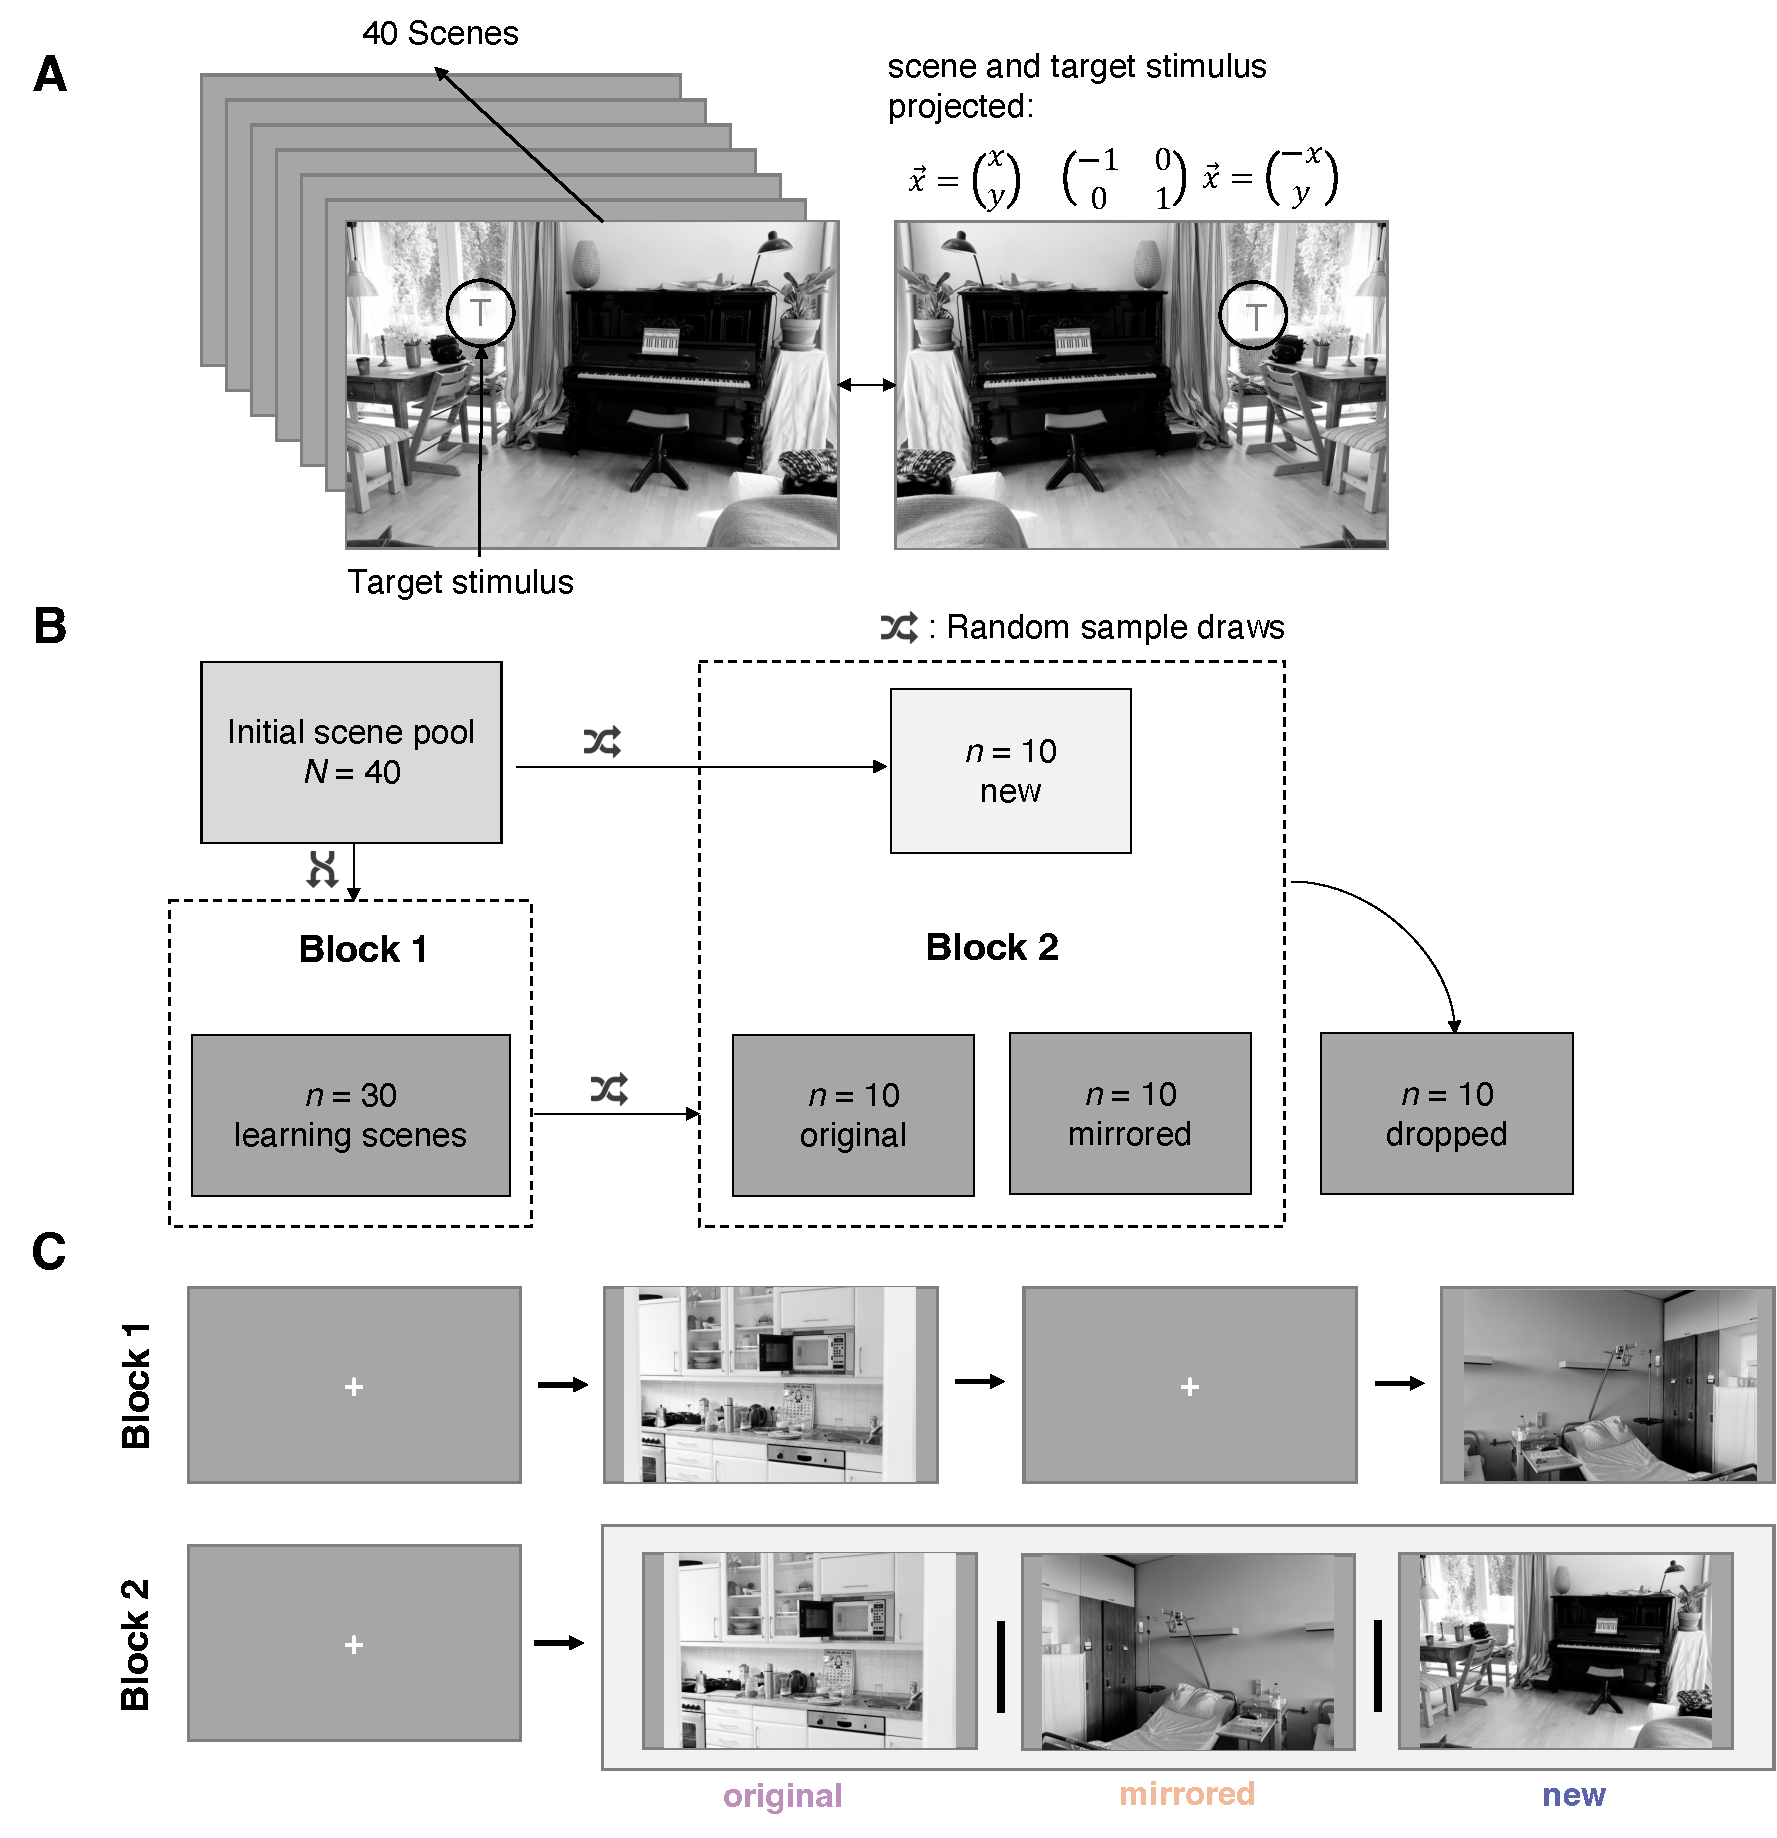
\includegraphics[width=0.7\linewidth]{../results/figures/experimental_design} 

}

\end{figure}


\begingroup
\footnotesize
\textit{Note:} \textbf{A}. 40 scenes of the BoIS dataset (Mohr et al., 2016) were chosen as the stimulus pool for the experiment. Participants were required to search a target stimulus (T) in each presented scene. For mirrored scenes in the second block, the target stimulus was also projected along the horizontal axis. \textbf{B}. From the initial 40 scenes, 30 scenes were randomly sampled for each participant in block 1. Subsequently, from these sampled scenes,  10 scenes were presented unmirrored (original) and mirrored respectively. To allow a baseline comparison, 10 new scenes that were not shown to the participants before, were included in block 2. \textbf{C}. All trial sequences started the presentation of a fixation cross and then continued in the aforementioned procedure.
\endgroup
\end{figure}

\hypertarget{design-and-procedure}{%
\subsection{Design and procedure}\label{design-and-procedure}}

In order to examine the adaption of contextual learning to spatial manipulation in real-world scenes, we implemented a 2x3 within-participant factorial design with the 2-level factor block (learning, testing) and 3-level factor orientation (new, mirrored, original). Both blocks comprised 30 trials yielding 60 trials in total. In the learning block, 30 scenes from the image pool of 40 scenes were randomly drawn and presented to the participants for the first time (see figure 1a). Participants transitioned fluently without notification from the learning to the testing block. As depicted in figure 1b, the 30 trials of the testing block were subdivided into new, original and mirrored trials, each consisting of 10 trials. In the new (baseline) trials, participants were shown scenes that were not presented previously in first block. Original trial scenes in the testing block consisted of 10 previously shown scenes that were presented with the identical invariant spatial layout. On the contrary, the mirrored testing trials were comprised the 10 previously shown scenes but this time mirrored together with the target along the x-axis (see figure 1a).

Before beginning the experiment, participants were introduced to the target stimulus and were given a description of the subsequent visual search task. After this, participants completed the aforementioned two blocks with 60 trials in total. Importantly, within each block, the three conditions were presented in random order to rule out any confounding sequence effects.

\hypertarget{data-analysis}{%
\subsection{Data analysis}\label{data-analysis}}

In the past decades, statistical techniques with more computational complexity such as multilevel linear mixed models (LMM) have become a prominent alternative in psychological research compared to more traditional approaches such as (repeated-measure) ANOVAs (Blanca, Alarc'on, \& Bono, 2018; Bono, Alarc'on, \& Blanca, 2021; Meteyard \& Davies, 2020). Concerning the present study, the use of the LMM offers at least two advantages over repeated-measures ANOVA. Firstly, LMM is able to elegantly account for the hierarchical nature of the non-independent data (Hox, Moerbeek, \& Schoot, 2017), by partioning the error variance and thus explicitly modeling the hierarchical structure (Harrison et al., 2018). Secondly, linear mixed models can deal with missing data more easily than repeated-measure ANOVA, which in turn can severely suffer from unbalanced data (Krueger \& Tian, 2004; Shaw \& Mitchell-Olds, 1993).

Considering these advantages, we implemented a linear mixed regression model in R (R. C. Team, 2022) within RStudio (Rs. Team, 2022) using mainly the \emph{lme4} package (Bates et al., 2022). We modeled the reaction time of the participants as the dependent variable and included fixed effects for the block and orientation factors as well their interaction. For both block and orientation, treatment contrasts were used to test the hypotheses with block 1 being the reference level for the former and the mirrored condition being the reference level for the latter. Moreover, we included the identifiers for each participant and scene as crossed random intercept effects (Baayen, Davidson, \& Bates, 2008) to account for the violation of independence within the participants and to consider the scenes as random samples from larger population pool of scenes. Model results were obtained using maximum likelihood (ML) and inference of the model parameters was drawn using parametric bootstrapping with percentile confidence intervals as implemented in the package \emph{lmeresampler} (see Loy \& Korobova, 2021). An overview of all important packages used for the analysis is included in the appendix.

\hypertarget{results}{%
\section{Results}\label{results}}

\hypertarget{descriptive-search-performance}{%
\subsection{Descriptive search performance}\label{descriptive-search-performance}}

The overall hit rate was 0.81. Regarding the hit rates between the different orientation conditions troughout the learning and testing block, table 1 indicates, that participants improved in performance in all 3 conditions. Concerning the descriptive response time trends, for both the baseline condition and the original condition, a decrease of reaction time was observable, indicating that the participants´ search time was faster in the second block compared to the first. However, for the mirrored condition, no decrease but instead a marginal increase in response time in block 2 was observable. Hence, visual search marginally worsened from block 1 to block 2 for mirrored scenes (see figure 2). The variances of the conditions reveal a similar pattern, in that for original and newly presented scenes, the variance decreases while for the mirrored condition, the variance increases troughout the two blocks.

\begin{onehalfspacing}
\begingroup\fontsize{10}{12}\selectfont

\begin{ThreePartTable}
\begin{TableNotes}[para]
\item \textit{\footnotesize{Note.}} 
\item \footnotesize{$n$: total number of hits in each condition, $M$: mean, $SD$: standard deviation.}
\end{TableNotes}
\begin{longtabu} to \linewidth {>{\raggedright}X>{\centering}X>{\centering}X>{\centering}X>{\centering}X>{\centering}X>{\centering}X}
\caption{\label{tab:unnamed-chunk-2}Descriptive table of the the reaction times and hit rates for each level of the two factors block and orientation}\\
\toprule
\multicolumn{1}{c}{ } & \multicolumn{3}{c}{Block 1} & \multicolumn{3}{c}{Block 2} \\
\cmidrule(l{3pt}r{3pt}){2-4} \cmidrule(l{3pt}r{3pt}){5-7}
\multicolumn{1}{c}{Orientation} & \multicolumn{1}{c}{$M$ ($SD$)} & \multicolumn{1}{c}{$n$} & \multicolumn{1}{c}{Hit rate} & \multicolumn{1}{c}{$M$  ($SD$) } & \multicolumn{1}{c}{$n$ } & \multicolumn{1}{c}{Hit rate }\\
\midrule
Original & 3.81 (3.27) & 74 & 0.82 & 2.96 (2.4) & 78 & 0.87\\
Mirrored & 3.68 (2.72) & 69 & 0.77 & 3.73 (2.87) & 75 & 0.83\\
New & 3.76 (2.9) & 67 & 0.74 & 3.25 (2.52) & 75 & 0.83\\
\bottomrule
\insertTableNotes
\end{longtabu}
\end{ThreePartTable}
\endgroup{}
\end{onehalfspacing}

\hypertarget{mixed-models-analysis}{%
\subsection{Mixed models analysis}\label{mixed-models-analysis}}

The summary of the fixed and random effects of the linear mixed model is depicted in table 2 With regard to the fixed effects, the grand intercept indicates that the mean reaction time of the mirrored scenes was 3.668 seconds, \(SE\) = 0.374, 95\% \(CI\) = {[}2.922, 4.412{]}. Regarding the main effect of block, the model estimated response times in the second block for the mirrored scenes to increase by 0.037 seconds relative to the first block (\(\beta_1\) = 0.037). For both orientation contrasts the mirrored condition was estimated to deviate positively from the new scenes (\(\beta_2\) = 0.12) and from the original scenes (\(\beta_3\) = 0.189). Most importantly with regard to the hypotheses, both interaction contrasts suggest that the response time differences between the first and second block were greater greater for both the repeated (\(\beta_4\) = -0.544) and novel (\(\beta_5\) = -0.89)) scenes when compared with the mirrored scenes. This is further illustrated in figure 3, which depicts the estimated marginal means. While the reponse times for both novel and repeated trials were estimated to decrease from block 1 to block 2, the response time of the mirrored scenes did not drop. However, when considering the inference of these effects, figure 4 shows, that all mentioned regression weights except the grand mean could not be supported inferentially as the confidence intervals enclose zero. Finally, regarding the random effects we derived the ICC based of the variances, which suggests that only 5.99\% of the variance could be explained by both variables.

\begin{onehalfspacing}
\begingroup\fontsize{10}{12}\selectfont

\begin{ThreePartTable}
\begin{TableNotes}[para]
\item \textit{\footnotesize{Note.}} 
\item \footnotesize{Significance was obtained using parametric bootstrapping with $n$ = 5000 resamples. If the 95 confidence interval ($CI$) encompasses zero, the regression weight is statistically non-significant. Because all predictors are discrete variables, treatment contrast coding was used (baseline for factor block: block 1, reference level for factor orientation: mirrored condition). Model fit: $L(\theta)$ = -1064.12, $AIC$ = 2146.24, $BIC$ = 2182.98, Deviance = 2128.24.}
\end{TableNotes}
\begin{longtabu} to \linewidth {>{\raggedright}X>{\centering}X>{\centering}X>{\centering}X>{\centering}X>{\centering}X}
\caption{\label{tab:unnamed-chunk-5}Summary of the linear mixed model results for the fixed effects of block and orientation as well as crossed random effects for participant and scene}\\
\toprule
\multicolumn{1}{c}{Term} & \multicolumn{1}{c}{Estimate} & \multicolumn{1}{c}{\textit{SE}} & \multicolumn{1}{c}{\textit{t}} & \multicolumn{1}{c}{95\% CI} & \multicolumn{1}{c}{Significance}\\
\midrule
\addlinespace[0.3em]
\multicolumn{6}{l}{Fixed}\\
\hspace{1em}Intercept $\beta_{0}$ & 3.668 & 0.374 & 9.803 & {}[2.922, 4.412] & $\ast$\\
\hspace{1em}Block $\beta_{1}$ & 0.037 & 0.449 & 0.083 & {}[-0.839, 0.927] & n.s.\\
\hspace{1em}Orient. $\beta_{2}$ & 0.12 & 0.467 & 0.257 & {}[-0.795, 1.059] & n.s.\\
\hspace{1em}Orient. $\beta_{3}$ & 0.189 & 0.457 & 0.414 & {}[-0.727, 1.082] & n.s.\\
\hspace{1em}Int. $\beta_{4}$ & -0.544 & 0.64 & -0.849 & {}[-1.836, 0.685] & n.s.\\
\hspace{1em}Int. $\beta_{5}$ & -0.89 & 0.626 & -1.421 & {}[-2.129, 0.326] & n.s.\\
\addlinespace[0.3em]
\multicolumn{6}{l}{Random}\\
\hspace{1em}$\sigma^{2}_{scene}$ & 0.209 & - & - & - & -\\
\hspace{1em}$\sigma^{2}_{participant}$ & 0.251 & - & - & - & -\\
\hspace{1em}$\sigma^{2}_{\epsilon}$ & 7.215 & - & - & - & -\\
\bottomrule
\insertTableNotes
\end{longtabu}
\end{ThreePartTable}
\endgroup{}
\end{onehalfspacing}

\hypertarget{discussion}{%
\section{Discussion}\label{discussion}}

The present study was set out with the aim to further investigate the nature of contextual information that guides attention in real-world scenes. In doing so, we examined if and to what extent reverse-mirroring of scenes together with the target stimulus affect learning in a contextual cueing paradigm. With regard to our first hypothesis, the results revealed that there is descriptive evidence that the benefit of contextual learning is greater for the invariant repeated scenes (original) relative to mirrored scenes. This manifested itself in a stronger decrease of response time for the repeated scenes from the learning to the testing block in comparison to the mirrored scenes. However, this descriptive evidence could not be supported inferentially. Contrary to our expectations, the direction of findings was even opposite to our second hypothesis. While a decrease in response time from the learning to the testing block was observed in the novel scenes, no decrease, but instead a marginal increase in response time was observed in the mirrored condition. Yet again, this opposing trend was not statistically significant.

The findings of the current study could neither replicate nor support the results of previous research (Brockmole \& Henderson, 2006a, 2006b). Altough the descriptive trends of the enhanced benefit of contextual learning for repeated scenes relative to mirrored scenes were in line with these studies, we found no inferential support to confirm the hypothesis. Concerning our second hypothesis, it was found that even the descriptive trend was opposing the results of Brockmole and Henderson (2006a). Wheras results of this study suggested that the search performance was still superior compared to the novel scenes, the descriptive trends of the present study indicated the opposite. When considered on a purely descriptive level, the results support the notion of previous studies showing that change of spatial contingencies between the target stimulus and the distractor environment can produce contextual cost (Conci \& Müller, 2012; Conci et al., 2011; Makovski \& Jiang, 2010). Though, these trends were only found descriptively and could not be supported inferentially. To further interprete these inconsistent findings, it is important to consider, that the present study did not find any general evidence of significant contextual learning. This might be explained by an inferior study design compared to traditional approaches, in which multiple learning blocks are typically implemented to establish the contextual cueing effect before manipulating the spatial layout (Jiang \& Sisk, 2020). Morover, supplementary analyses (see appendix) showed clear evidence of non-accounted influence of perceptual scene aspects like contrast on the response time performance. Lastly, the present study was limited to a very small sample size, which contributes to a very poor power in addition to the small number of blocks.

With these limitations in mind, a follow-up study should incorporate several methodological considerations in addition to newly gained content suggestions. In the following section, both dimensions will be briefly discussed before a final synthesis is drawn.

As mentioned earlier, given the limited resources of the seminar, the present study used a design with only one learning block and one testing block that included the experimental manipulation. Consequently, we have implicitly assumed that after only one learning block, contextual learning effects have already been established in order to succeed in the subsequent manipulation. Altough, contextual associations between targets and scene properties emerge rapidly (Chun, 2003; Goujon et al., 2015), typical recommendations advocate for at least 30 blocks for a solid learning effect before the manipulation (Jiang \& Sisk, 2020). Together with aquiring more participants for a follow-up experiment, following up on these recommendations would yield higher power. Building on this, it is generally also advisable to carry out a power analysis (Jiang \& Sisk, 2020) from a pilot study. Regarding this, recent developed resources offer a feasable implementation in the framwork of mixed models (Kumle, Võ, \& Draschkow, 2021). Another important aspect that should be considered in a follow-up study stems from the results of the additional analysis. The clear evidence of the influence of contrast as a perceptual aspect of the scene on response time should encourage an attempt to control for this possible confound in a follow-up study. One possibility could be to adjust the contrast using RGB transformations that decrease the luminance difference of the image pixels. Finally and most importantly, limiting the experiment to over-simplified behavioral outcomes of visual search such as motor response times, precludes one from gaining more insightful results, that could be obtained via eye-tracking. Using eye-tracking in a follow-up study could be especially promising because of its potential ability to further characterise the complex dynamics between different contextual aspects of a scene and how these aspects interplay to guide attention.

In addition to the methodological considerations, the study also raised new content-wise research questions that could be expand upon. Firstly, because of the previously mentioned methodological limitations that should be adressed in a follow-up study, it would be sensible to incorporate the same manipulation that was employed in the present study, to verify, if there is still no support for the formulated hypotheses or if this was a confound of the poor study design. As mentioned previously, this could be especially insightful in combination with the implementation of eye-tracking. If the context providing information of real-scenes would be mainly determined by its semantic aspects, it would be likely that the gaze initially shifts towards the old target position. If however, more low-level aspects of the scene like spatial object relations would guide attention, it could be expected that gaze remains unaffected as the relative spatial relationships between objects remain constant in the mirrored condition (see Brockmole \& Henderson, 2006a). Additionally, a follow-up study could include a different variant of the mirror-reversal manipulation. Whereas in the present study, both the scene and the target stimulus were mirrored, a meaningful modification could entail the mirroring of the scene while keeping the target stimulus constant in position. Compared to the discussed overall inflexibility to \emph{relearning} of spatial contingencies in artificial stimulus-arrays (Conci \& Müller, 2012; Conci et al., 2011; Makovski \& Jiang, 2010; Zellin et al., 2013), the ability to adapt to such changes in real scenes remains largely unknown. By implementing this manipulation, this research question could be further examined. Finally, it would be recommended to include a recognition test at the end of the experiment to examine whether the memory expliciteness that previous studies argued for (Brockmole \& Henderson, 2006a, 2006b) can be further supported. This could be either implemented with a configuration recognition or a target generation task (see Jiang \& Sisk, 2020).

\hypertarget{conclusion}{%
\section{Conclusion}\label{conclusion}}

Despite the non-significant results of the present study, we seek to stimulate further investigation of contextual learning in real-world scenes by outlining considerations for future research. Most importantly, with respect to methodological aspects this should entail a larger number of learning blocks, the implementation of eye-tracking as well as aim to control for potentially confounding perceptual aspects of real-world scenes. Contentwise, we particularly emphasise the importance of examining the adapation of contextual learning to permanent spatial contingency changes in real-world scenes.

\newpage

\hypertarget{references}{%
\section{References}\label{references}}

\hypertarget{refs}{}
\begin{CSLReferences}{1}{0}
\leavevmode\vadjust pre{\hypertarget{ref-allaire_rmarkdown_2022}{}}%
Allaire, J. J., Xie {[}aut, Y., cre, McPherson, J., Luraschi, J., Ushey, K., \ldots{} filter), A. K. (pagebreak. L. (2022). \emph{Rmarkdown: {Dynamic} {Documents} for {R}}. Retrieved from \url{https://CRAN.R-project.org/package=rmarkdown}

\leavevmode\vadjust pre{\hypertarget{ref-aust_papaja_2022}{}}%
Aust, F., Barth, M., Diedenhofen, B., Stahl, C., Casillas, J. V., \& Siegel, R. (2022). \emph{Papaja: {Prepare} {American} {Psychological} {Association} {Journal} {Articles} with {R} {Markdown}}. Retrieved from \url{https://CRAN.R-project.org/package=papaja}

\leavevmode\vadjust pre{\hypertarget{ref-baayen_mixed-effects_2008}{}}%
Baayen, R. H., Davidson, D. J., \& Bates, D. M. (2008). Mixed-effects modeling with crossed random effects for subjects and items. \emph{Special Issue: Emerging Data Analysis}, \emph{59}(4), 390--412. \url{https://doi.org/10.1016/j.jml.2007.12.005}

\leavevmode\vadjust pre{\hypertarget{ref-bates_lme4_2022}{}}%
Bates, D., Maechler, M., Bolker, B., Walker, S., Christensen, R. H. B., Singmann, H., \ldots{} Krivitsky, P. N. (2022). \emph{lme4: {Linear} {Mixed}-{Effects} {Models} using '{Eigen}' and {S4}}. Retrieved from \url{https://CRAN.R-project.org/package=lme4}

\leavevmode\vadjust pre{\hypertarget{ref-blanca_current_2018}{}}%
Blanca, M. J., Alarc'on, R., \& Bono, R. (2018). Current {Practices} in {Data} {Analysis} {Procedures} in {Psychology}: {What} {Has} {Changed}? \emph{Frontiers in Psychology}, \emph{9}. Retrieved from \url{https://www.frontiersin.org/articles/10.3389/fpsyg.2018.02558}

\leavevmode\vadjust pre{\hypertarget{ref-bolker_broommixed_2022}{}}%
Bolker, B., Robinson, D., Menne, D., Gabry, J., Buerkner, P., Hua, C., \ldots{} Brunson, C. (2022). \emph{Broom.mixed: {Tidying} {Methods} for {Mixed} {Models}}. Retrieved from \url{https://CRAN.R-project.org/package=broom.mixed}

\leavevmode\vadjust pre{\hypertarget{ref-bono_report_2021}{}}%
Bono, R., Alarc'on, R., \& Blanca, M. J. (2021). Report {Quality} of {Generalized} {Linear} {Mixed} {Models} in {Psychology}: {A} {Systematic} {Review}. \emph{Frontiers in Psychology}, \emph{12}. Retrieved from \url{https://www.frontiersin.org/articles/10.3389/fpsyg.2021.666182}

\leavevmode\vadjust pre{\hypertarget{ref-brockmole_contextual_2006}{}}%
Brockmole, J. R., Castelhano, M. S., \& Henderson, J. M. (2006). Contextual cueing in naturalistic scenes: {Global} and local contexts. \emph{Journal of Experimental Psychology: Learning, Memory, and Cognition}, \emph{32}, 699--706. \url{https://doi.org/10.1037/0278-7393.32.4.699}

\leavevmode\vadjust pre{\hypertarget{ref-brockmole_recognition_2006}{}}%
Brockmole, J. R., \& Henderson, J. M. (2006a). Recognition and attention guidance during contextual cueing in real-world scenes: {Evidence} from eye movements. \emph{The Quarterly Journal of Experimental Psychology}, \emph{59}(7), 1177--1187. \url{https://doi.org/10.1080/17470210600665996}

\leavevmode\vadjust pre{\hypertarget{ref-brockmole_using_2006}{}}%
Brockmole, J. R., \& Henderson, J. M. (2006b). Using real-world scenes as contextual cues for search. \emph{Visual Cognition}, \emph{13}(1), 99--108. \url{https://doi.org/10.1080/13506280500165188}

\leavevmode\vadjust pre{\hypertarget{ref-chun_contextual_2000}{}}%
Chun, M. M. (2000). Contextual cueing of visual attention. \emph{Trends in Cognitive Sciences}, \emph{4}(5), 170--178. \url{https://doi.org/10.1016/S1364-6613(00)01476-5}

\leavevmode\vadjust pre{\hypertarget{ref-chun_scene_2003}{}}%
Chun, M. M. (2003). Scene {Perception} and {Memory}. In \emph{Cognitive {Vision}}: \emph{Vol.} \emph{42}. \emph{Psychology of {Learning} and {Motivation}} (pp. 79--108). Academic Press. \url{https://doi.org/10.1016/S0079-7421(03)01003-X}

\leavevmode\vadjust pre{\hypertarget{ref-chun_contextual_1998}{}}%
Chun, M. M., \& Jiang, Y. (1998). Contextual {Cueing}: {Implicit} {Learning} and {Memory} of {Visual} {Context} {Guides} {Spatial} {Attention}. \emph{Cognitive Psychology}, \emph{36}(1), 28--71. \url{https://doi.org/10.1006/cogp.1998.0681}

\leavevmode\vadjust pre{\hypertarget{ref-conci_contextual_2012}{}}%
Conci, M., \& Müller, H. J. (2012). Contextual learning of multiple target locations in visual search. \emph{Visual Cognition}, \emph{20}(7), 746--770. \url{https://doi.org/10.1080/13506285.2012.694376}

\leavevmode\vadjust pre{\hypertarget{ref-conci_contextual_2011}{}}%
Conci, M., Sun, L., \& Müller, H. J. (2011). Contextual remapping in visual search after predictable target-location changes. \emph{Psychological Research}, \emph{75}(4), 279--289. \url{https://doi.org/10.1007/s00426-010-0306-3}

\leavevmode\vadjust pre{\hypertarget{ref-goujon_investigating_2015}{}}%
Goujon, A., Didierjean, A., \& Thorpe, S. (2015). Investigating implicit statistical learning mechanisms through contextual cueing. \emph{Trends in Cognitive Sciences}, \emph{19}(9), 524--533. \url{https://doi.org/10.1016/j.tics.2015.07.009}

\leavevmode\vadjust pre{\hypertarget{ref-harrison_brief_2018}{}}%
Harrison, X., Donaldson, L., Correa, M., Evans, J., Fisher, D., Goodwin, C., \ldots{} Inger, R. (2018). A brief introduction to mixed effects modelling and multi-model inference in ecology. \emph{PeerJ}, \emph{6}, e4794. \url{https://doi.org/10.7717/peerj.4794}

\leavevmode\vadjust pre{\hypertarget{ref-henderson_high-level_1999}{}}%
Henderson, J. M., \& Hollingworth, A. (1999). High-level scene perception. \emph{Annual Review of Psychology}, \emph{50}(1), 243--271. \url{https://doi.org/10.1146/annurev.psych.50.1.243}

\leavevmode\vadjust pre{\hypertarget{ref-henry_purrr_2022}{}}%
Henry, L., \& Wickham, H. (2022). \emph{Purrr: {Functional} {Programming} {Tools}}. Retrieved from \url{https://CRAN.R-project.org/package=purrr}

\leavevmode\vadjust pre{\hypertarget{ref-hox_multilevel_2017}{}}%
Hox, J., Moerbeek, M., \& Schoot, R. van de. (2017). \emph{Multilevel {Analysis}: {Techniques} and {Applications}} (3rd ed.). New York: Routledge. \url{https://doi.org/10.4324/9781315650982}

\leavevmode\vadjust pre{\hypertarget{ref-jiang_contextual_2020}{}}%
Jiang, Y. V., \& Sisk, C. A. (2020). Contextual {Cueing}. In S. Pollmann (Ed.), \emph{Spatial {Learning} and {Attention} {Guidance}} (pp. 59--72). New York, NY: Springer US. \url{https://doi.org/10.1007/7657_2019_19}

\leavevmode\vadjust pre{\hypertarget{ref-kay_ggdist_2022}{}}%
Kay, M., \& Wiernik, B. M. (2022). \emph{Ggdist: {Visualizations} of {Distributions} and {Uncertainty}}. Retrieved from \url{https://CRAN.R-project.org/package=ggdist}

\leavevmode\vadjust pre{\hypertarget{ref-krueger_comparison_2004}{}}%
Krueger, C., \& Tian, L. (2004). A {Comparison} of the {General} {Linear} {Mixed} {Model} and {Repeated} {Measures} {ANOVA} {Using} a {Dataset} with {Multiple} {Missing} {Data} {Points}. \emph{Biological Research For Nursing}, \emph{6}(2), 151--157. \url{https://doi.org/10.1177/1099800404267682}

\leavevmode\vadjust pre{\hypertarget{ref-kuhn_multilevelmod_2022}{}}%
Kuhn, M., Frick, H., \& RStudio. (2022). \emph{Multilevelmod: {Model} {Wrappers} for {Multi}-{Level} {Models}}. Retrieved from \url{https://CRAN.R-project.org/package=multilevelmod}

\leavevmode\vadjust pre{\hypertarget{ref-kuhn_tidymodels_2022}{}}%
Kuhn, M., \& Wickham, H. (2022). \emph{Tidymodels: {Easily} {Install} and {Load} the '{Tidymodels}' {Packages}}. Retrieved from \url{https://CRAN.R-project.org/package=tidymodels}

\leavevmode\vadjust pre{\hypertarget{ref-kumle_estimating_2021}{}}%
Kumle, L., Võ, M. L.-H., \& Draschkow, D. (2021). Estimating power in (generalized) linear mixed models: {An} open introduction and tutorial in {R}. \emph{Behavior Research Methods}, \emph{53}(6), 2528--2543. \url{https://doi.org/10.3758/s13428-021-01546-0}

\leavevmode\vadjust pre{\hypertarget{ref-loy_bootstrapping_2021}{}}%
Loy, A., \& Korobova, J. (2021). \emph{Bootstrapping {Clustered} {Data} in {R} using lmeresampler}. arXiv. \url{https://doi.org/10.48550/arXiv.2106.06568}

\leavevmode\vadjust pre{\hypertarget{ref-makovski_contextual_2010}{}}%
Makovski, T., \& Jiang, Y. V. (2010). Contextual cost: {When} a visual-search target is not where it should be. \emph{Quarterly Journal of Experimental Psychology}, \emph{63}(2), 216--225. \url{https://doi.org/10.1080/17470210903281590}

\leavevmode\vadjust pre{\hypertarget{ref-manginelli_misleading_2009}{}}%
Manginelli, A. A., \& Pollmann, S. (2009). Misleading contextual cues: {How} do they affect visual search? \emph{Psychological Research}, \emph{73}(2), 212--221. \url{https://doi.org/10.1007/s00426-008-0211-1}

\leavevmode\vadjust pre{\hypertarget{ref-meteyard_best_2020}{}}%
Meteyard, L., \& Davies, R. A. I. (2020). Best practice guidance for linear mixed-effects models in psychological science. \emph{Journal of Memory and Language}, \emph{112}, 104092. \url{https://doi.org/10.1016/j.jml.2020.104092}

\leavevmode\vadjust pre{\hypertarget{ref-mohr_boisberlin_2016}{}}%
Mohr, J., Seyfarth, J., Lueschow, A., Weber, J. E., Wichmann, F. A., \& Obermayer, K. (2016). {BOiS}---{Berlin} {Object} in {Scene} {Database}: {Controlled} {Photographic} {Images} for {Visual} {Search} {Experiments} with {Quantified} {Contextual} {Priors}. \emph{Frontiers in Psychology}, \emph{7}. Retrieved from \url{https://www.frontiersin.org/articles/10.3389/fpsyg.2016.00749}

\leavevmode\vadjust pre{\hypertarget{ref-oliva_role_2007}{}}%
Oliva, A., \& Torralba, A. (2007). The role of context in object recognition. \emph{Trends in Cognitive Sciences}, \emph{11}, 520--527. \url{https://doi.org/10.1016/j.tics.2007.09.009}

\leavevmode\vadjust pre{\hypertarget{ref-peirce_building_2022}{}}%
Peirce, J. W., Hirst, R. J., \& MacAskill, M. R. (2022). \emph{Building {Experiments} in {PsychoPy}} (2nd ed.). Sage.

\leavevmode\vadjust pre{\hypertarget{ref-peirce_psychopy2_2019}{}}%
Peirce, J., Gray, J. R., Simpson, S., MacAskill, M., Höchenberger, R., Sogo, H., \ldots{} Lindeløv, J. K. (2019). {PsychoPy2}: {Experiments} in behavior made easy. \emph{Behavior Research Methods}, \emph{51}(1), 195--203. \url{https://doi.org/10.3758/s13428-018-01193-y}

\leavevmode\vadjust pre{\hypertarget{ref-rosenbaum_interaction_2013}{}}%
Rosenbaum, G. M., \& Jiang, Y. V. (2013). Interaction between scene-based and array-based contextual cueing. \emph{Attention, Perception, \& Psychophysics}, \emph{75}(5), 888--899. \url{https://doi.org/10.3758/s13414-013-0446-9}

\leavevmode\vadjust pre{\hypertarget{ref-shaw_anova_1993}{}}%
Shaw, R. G., \& Mitchell-Olds, T. (1993). Anova for {Unbalanced} {Data}: {An} {Overview}. \emph{Ecology}, \emph{74}(6), 1638--1645. \url{https://doi.org/10.2307/1939922}

\leavevmode\vadjust pre{\hypertarget{ref-r_core_team_r_2022}{}}%
Team, R. C. (2022). \emph{R: {A} language and environment for statistical computing}. Vienna, Austria: R Foundation for Statistical Computing. Retrieved from \url{https://www.R-project.org/}

\leavevmode\vadjust pre{\hypertarget{ref-rstudio_team_rstudio_2022}{}}%
Team, Rs. (2022). \emph{{RStudio}: {Integrated} {Development} {Environment} for {R}}. Boston, MA: RStudio, PBC. Retrieved from \url{http://www.rstudio.com/.}

\leavevmode\vadjust pre{\hypertarget{ref-tiedemann_gghalves_2022}{}}%
Tiedemann, F. (2022). \emph{Gghalves: {Compose} {Half}-{Half} {Plots} {Using} {Your} {Favourite} {Geoms}}. Retrieved from \url{https://CRAN.R-project.org/package=gghalves}

\leavevmode\vadjust pre{\hypertarget{ref-wickham_stringr_2022}{}}%
Wickham, H. (2022). \emph{Stringr: {Simple}, {Consistent} {Wrappers} for {Common} {String} {Operations}}. Retrieved from \url{https://CRAN.R-project.org/package=stringr}

\leavevmode\vadjust pre{\hypertarget{ref-wickham_ggplot2_2022}{}}%
Wickham, H., Chang, W., Henry, L., Pedersen, T. L., Takahashi, K., Wilke, C., \ldots{} Dunnington, D. (2022). \emph{ggplot2: {Create} {Elegant} {Data} {Visualisations} {Using} the {Grammar} of {Graphics}}. Retrieved from \url{https://CRAN.R-project.org/package=ggplot2}

\leavevmode\vadjust pre{\hypertarget{ref-wickham_dplyr_2022}{}}%
Wickham, H., François, R., Henry, L., \& Müller, K. (2022). \emph{Dplyr: {A} {Grammar} of {Data} {Manipulation}}. Retrieved from \url{https://CRAN.R-project.org/package=dplyr}

\leavevmode\vadjust pre{\hypertarget{ref-wilke_ggridges_2022}{}}%
Wilke, C. O. (2022). \emph{Ggridges: {Ridgeline} {Plots} in 'ggplot2'}. Retrieved from \url{https://CRAN.R-project.org/package=ggridges}

\leavevmode\vadjust pre{\hypertarget{ref-wilke_ggtext_2022}{}}%
Wilke, C. O., \& Wiernik, B. M. (2022). \emph{Ggtext: {Improved} {Text} {Rendering} {Support} for 'ggplot2'}. Retrieved from \url{https://CRAN.R-project.org/package=ggtext}

\leavevmode\vadjust pre{\hypertarget{ref-xie_knitr_2022}{}}%
Xie, Y., Sarma, A., Vogt, A., Andrew, A., Zvoleff, A., Al-Zubaidi, A., \ldots{} Kamvar, Z. N. (2022). \emph{Knitr: {A} {General}-{Purpose} {Package} for {Dynamic} {Report} {Generation} in {R}}. Retrieved from \url{https://CRAN.R-project.org/package=knitr}

\leavevmode\vadjust pre{\hypertarget{ref-zellin_here_2013}{}}%
Zellin, M., Conci, M., Mühlenen, A. von, \& Müller, H. J. (2013). Here {Today}, {Gone} {Tomorrow} -- {Adaptation} to {Change} in {Memory}-{Guided} {Visual} {Search}. \emph{PLOS ONE}, \emph{8}(3), e59466. \url{https://doi.org/10.1371/journal.pone.0059466}

\end{CSLReferences}

\newpage

\hypertarget{appendix}{%
\section{Appendix}\label{appendix}}

\hypertarget{study-contributions}{%
\subsection{Study contributions}\label{study-contributions}}

\noindent Study design \& data aquisition: Annika Böhler, Zarah Schreiner, Katharina Scholz and Jan Luca Schnatz; analysis \& manuscript: Jan Luca Schnatz

\hypertarget{fair-data-statement}{%
\subsection{FAIR data statement}\label{fair-data-statement}}

All raw data as well as analyses scripts are made available under the public MIT license for reuse via GitHub: \url{https://github.com/jlschnatz/scene_orientation_contextual_cueing}

\noindent List of the main packages used for the analyses:

\begin{itemize}
\tightlist
\item
  data manipulation: \emph{dplyr} (Wickham, François, Henry, \& Müller, 2022), \emph{purrr} (Henry \& Wickham, 2022), \emph{stringr} (Wickham, 2022)
\item
  data modeling: \emph{lme4} (Bates et al., 2022), \emph{tidymodels} (Kuhn \& Wickham, 2022), \emph{multilevelmod} (Kuhn, Frick, \& RStudio, 2022), \emph{broom.mixed} (Bolker et al., 2022), \emph{lmeresampler} (Loy \& Korobova, 2021)
\item
  data visualization: \emph{ggplot2} (Wickham et al., 2022), \emph{ggridges} (Wilke, 2022), \emph{ggdist} (Kay \& Wiernik, 2022), \emph{gghalves} (Tiedemann, 2022), \emph{ggtext} (Wilke \& Wiernik, 2022)
\item
  reporting: \emph{papaja} (Aust et al., 2022), \emph{knitr} (Xie et al., 2022), \emph{rmarkdown} (Allaire et al., 2022)
\end{itemize}

\newpage

\begin{figure}[H]

\begin{figure}

\caption{Descriptive reaction time differences between the learning and testing block for each condition (new, original and mirrored)
\label{fig:rt-diff}}

{\centering 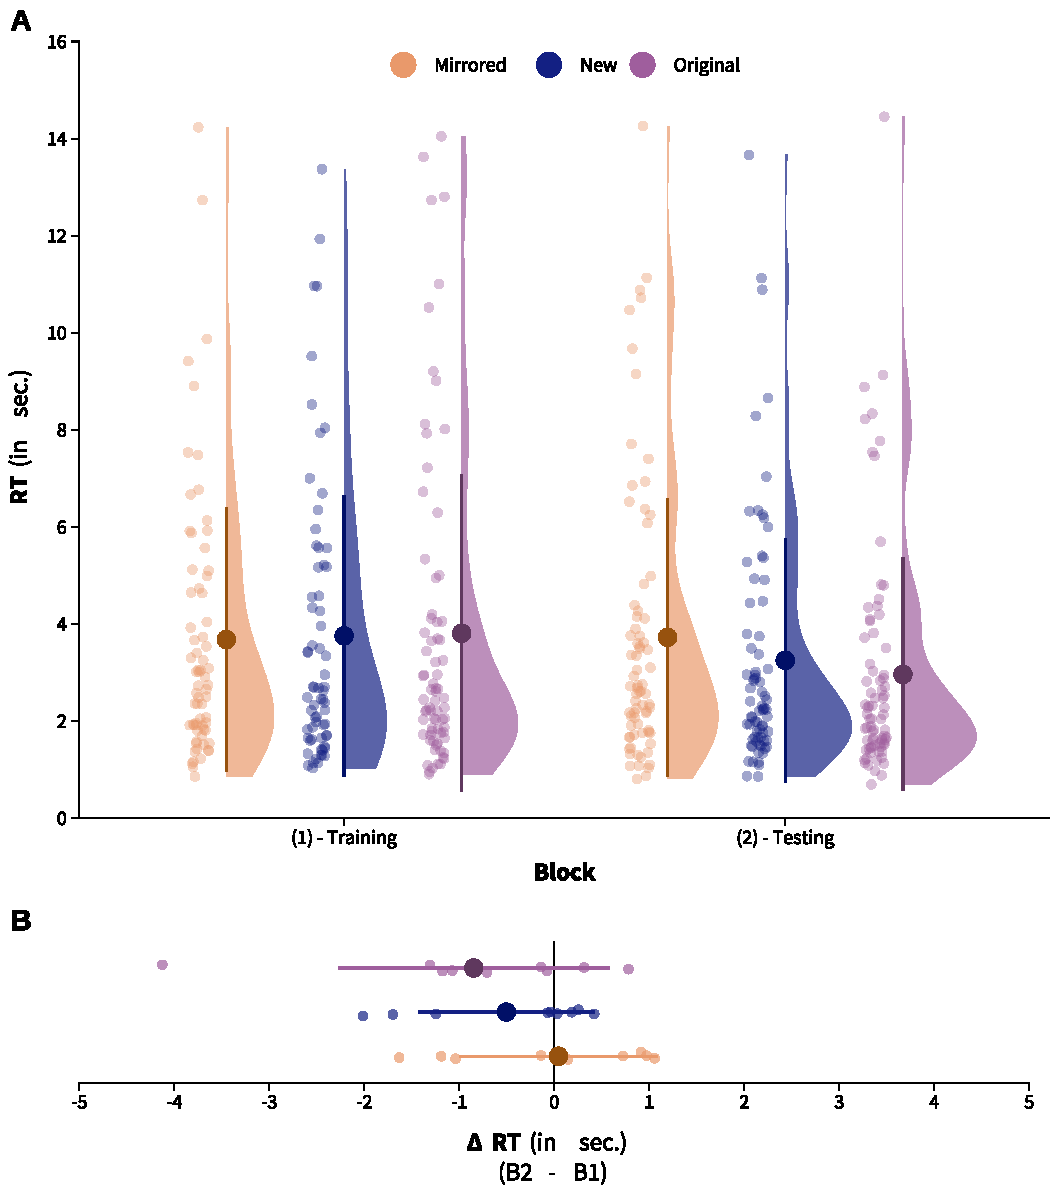
\includegraphics[width=0.7\linewidth]{../results/figures/combined_rt_diff} 

}

\end{figure}


\begingroup
\footnotesize
\textit{Note:} \textbf{A}. Figure displays the density distributions for each level of the two conditions block and orientation, as well as the jittered raw data points. The pointrange indicates the mean reaction time (RT) in each condition as well as the lower and upper SEM. \textbf{B}. Figure displays the aggregated reaction time differences between block 2 and block 1 (B2 - B1) for each participant. Negative values consequently indicate, that the reaction time was lower in block 2 compared to block 1.
\endgroup
\end{figure}

\begin{figure}[H]

\begin{figure}

\caption{Estimated marginal means of the linear mixed models for the factors block and orientation)
\label{fig:marginal-mean}}

{\centering 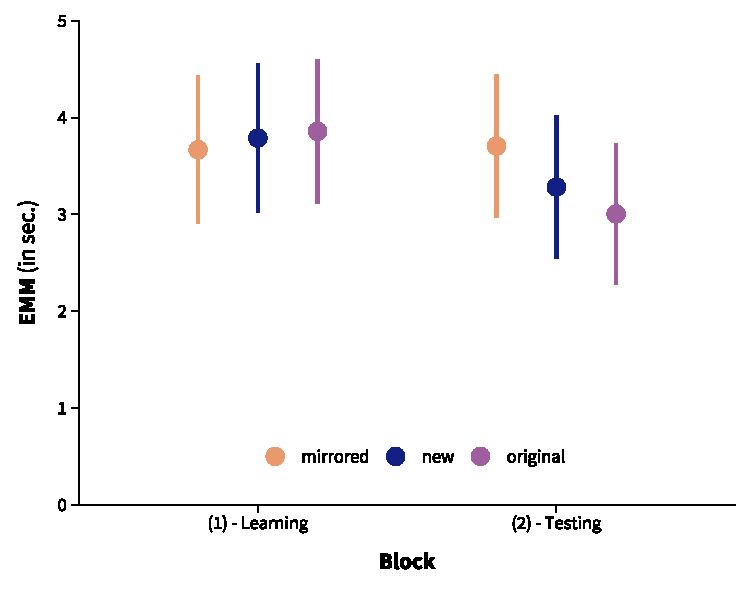
\includegraphics[width=0.7\linewidth]{../results/figures/marginal_means} 

}

\end{figure}


\begingroup
\footnotesize
\textit{Note:} EMM: estimated marginal mean. Vertical linerange indicates the standard error.
\endgroup
\end{figure}

\begin{figure}[H]

\begin{figure}

\caption{Inference estimates for the fixed regression coefficients of the LMM using parametric bootstrapping. \label{fig:bootstrap}}

{\centering 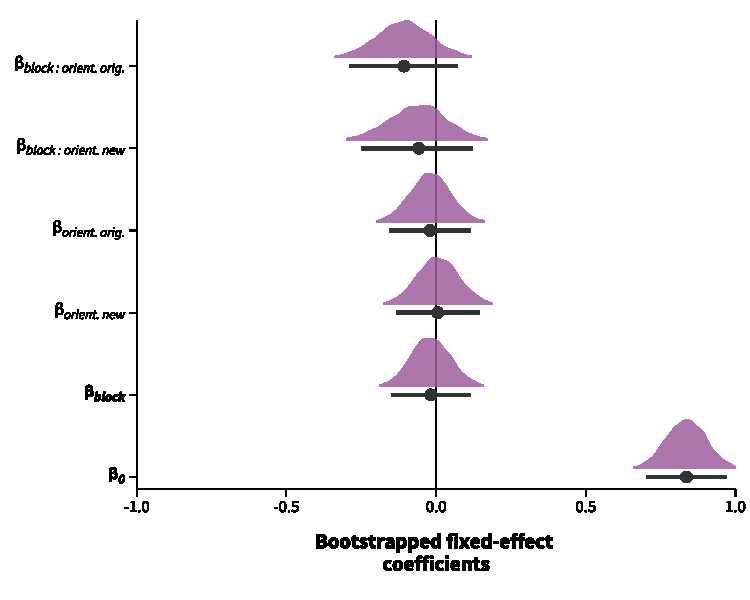
\includegraphics[width=0.8\linewidth]{../results/figures/bootstrapped_weights} 

}

\end{figure}


\begingroup
\footnotesize
\textit{Note:} Parametric bootstrap sample size was $B$ = 5000. Confidence intervals were obtained using two sided percentile bootstrapping with  $\alpha$ = 0.05.
\endgroup
\end{figure}

\newpage

\newpage

\hypertarget{supplementary-analysis}{%
\subsection{Supplementary analysis}\label{supplementary-analysis}}

After completing the experiment, numerous participants stated they had the impression, the search task was strongly influenced by the contrast difference between the target stimulus and the background of the scene. This opened up the question of possible non-controlled merely perceptual visibility effects. To further investigate this question, we derived two perceptual aspects between the scene and the target stimulus, namely the center distance and the contrast difference. The center distance was defined as the euclidean distance between the target and the center fixation point. The contrast distance was derived as the mean absolute difference between the target stimulus RGB-value and the RGB-values from a circular window around the target of with a radius of \(r\) = .08 (height units). Although the more reliable choice of the parameter \(r\) should be made by simulation, this specification ensures that the nearest context around the stimulus is taken into account and should thus be able to reveal initial insights. We fitted and regular LMM and a GLMM model using ML, each with the two mentioned normalized predictors as fixed effects and participants as random effects, the former predicting the response time and the latter predicting, whether a single trial was a hit or miss (logistic mixed model). Significance was obtained using the same bootstrapping approach of the main model.

As depicted in table 3 in both models the effect of the contrast was estimated to be statistically significant while the effect of the distance from the center was estimated to be statistically non-significant. The regression weight for the contrast in the GLMM model was positive (\(\beta_{contrast}\) = 0.784, \(OR\) = 2.19) indicating, that the increase of 1 \emph{SD} in contrast multiplies the odds of a hit by 2.19. Similarly, the negative weight for the contrast in the LMM model (\(\beta_{contrast}\) = -0.274) indicates that for every 1 \emph{SD} increase in contrast, the response time decreases by an average of -0.274 seconds.

\newpage

\begin{onehalfspacing}
\begingroup\fontsize{10}{12}\selectfont

\begin{ThreePartTable}
\begin{TableNotes}[para]
\item \textit{\footnotesize{Note.}} 
\item \footnotesize{Model fit LMM: L($\theta$) = -1065.46, $AIC$ = 2140.91, $BIC$ = 2161.32, Deviance = 2130.91. Model fit GLMM: L($\theta$) = -239.86, $AIC$ = 487.73, $BIC$ = 504.89, Deviance = 468.33}
\end{TableNotes}
\begin{longtabu} to \linewidth {>{\raggedright}X>{\centering}X>{\centering}X>{\centering}X>{\centering}X>{\centering}X>{\centering}X>{\centering}X>{\centering}X>{\centering}X>{\centering}X}
\caption{\label{tab:unnamed-chunk-9}Summary of the logistic and linear mixed model that predicted hit and response time by contrast and center distance}\\
\toprule
\multicolumn{1}{c}{\em{ }} & \multicolumn{5}{c}{\em{GLMM: Hit/Miss}} & \multicolumn{5}{c}{\em{LMM: Reaction Time}} \\
\cmidrule(l{3pt}r{3pt}){2-6} \cmidrule(l{3pt}r{3pt}){7-11}
\multicolumn{1}{c}{Term} & \multicolumn{1}{c}{Estimate} & \multicolumn{1}{c}{$SE$} & \multicolumn{1}{c}{$z$} & \multicolumn{1}{c}{$CI$} & \multicolumn{1}{c}{Signif.} & \multicolumn{1}{c}{Estimate } & \multicolumn{1}{c}{$SE$ } & \multicolumn{1}{c}{$t$ } & \multicolumn{1}{c}{$CI$ } & \multicolumn{1}{c}{Signif. }\\
\midrule
$\beta_{0}$ & 1.673 & 0.179 & 9.328 & {}[1.339, 2.055] & $\ast$ & 3.559 & 0.209 & 17.045 & {}[3.147, 3.972] & $\ast$\\
$\beta_{distance}$ & 0.088 & 0.116 & 0.759 & {}[-0.141, 0.319] & n.s. & 0.151 & 0.133 & 1.137 & {}[-0.11, 0.41] & n.s.\\
$\beta_{contrast}$ & 0.784 & 0.134 & 5.86 & {}[0.539, 1.055] & $\ast$ & -0.274 & 0.134 & -2.054 & {}[-0.537, -0.014] & $\ast$\\
$\sigma^{2}_{subj.}$ & 0.133 & - & - & - & - & 0.236 & - & - & - & -\\
$\sigma^{2}_{\epsilon}$ & - & - & - & - & - & 7.449 & - & - & - & -\\
\bottomrule
\insertTableNotes
\end{longtabu}
\end{ThreePartTable}
\endgroup{}
\end{onehalfspacing}


\end{document}
